% MICA final report draft — every claim mapped to its banked data (2026-07-19)
% Compile: .\tools\tectonic.exe report.tex
\documentclass[11pt]{article}
\usepackage[margin=1.1in]{geometry}
\usepackage{amsmath}
\usepackage{pgfplots}
\pgfplotsset{compat=1.17,
  every node near coord/.append style={/pgf/number format/fixed,
    /pgf/number format/precision=3}}
\usepackage{booktabs}
\usepackage{caption}
\definecolor{micablue}{RGB}{46,110,180}
\definecolor{micagray}{RGB}{140,140,140}
\definecolor{micagreen}{RGB}{60,145,90}
\definecolor{micared}{RGB}{180,70,60}

\title{MICA: Measuring Whether an AI Can Understand a Builder's\\
Situation and Intentions from Raw Observation}
\author{Benjamin [surname] \\ \small [institution, program]}
\date{July 2026 --- draft}

\begin{document}
\maketitle

\begin{abstract}
Can an AI watching a person build recognize what is being made and anticipate
what comes next --- from raw observation alone, with no instructions and no
privileged game state? I built and instrumented a full pipeline for this
question in Minecraft: frozen 2D foundation-model features (VPT, MineCLIP) and
frozen 3D shape embeddings (Uni3D) feed a Bayesian belief over building goals,
which gates an embodied assistant. The claim of this thesis is not that the
system ``understands''; it is that I built an honest measurement apparatus for
that question and report what it measured. Five results stand: intent inference
is \emph{necessary} once builds leave templates (a structure-only baseline
collapses to 0.042 final-goal accuracy on 24 never-seen real sessions while the
belief tracker holds 0.375, chance 0.2); the system anticipates a builder's
next actions far above chance (71\% next-action, 59\% eight-actions-ahead
token accuracy vs.\ 1.2\% chance, on held-out real sessions); structural
understanding accumulates lawfully with observation (partial-view embeddings
converge to 0.92 cosine with the full structure); the system improves lawfully
with the right data (two pre-registered experiments, both won); and the
apparatus itself is trustworthy --- its falsification criteria fired, a feature
leak was found and a published verdict honestly reversed, and every negative is
banked. Equally important are the claims I do \emph{not} make: early
recognition is statistically unproven, confidence is uncalibrated, the belief
adds no measurable prediction fuel, and the agent has never placed a block ---
assistance is designed and safety-gated, never evaluated.
\end{abstract}

\section{Introduction: why this question}

In structured work environments --- construction sites, warehouses, assembly
lines --- an assistant that must be \emph{told} everything is bottlenecked by
the telling. The expensive resource is the human's attention, not the robot's
labor. Cooperative inverse reinforcement learning formalized this a decade ago
\cite{cirl}: assistance without explicit instruction is a game in which the
helper must infer the human's hidden objective, and the belief over that
objective is the object everything else depends on. Benchmarks built on that
frame established both directions of the necessity argument: goal-agnostic
helping fails, and a confidently wrong helper is \emph{worse than none} ---
undoing the human's work in 40\% of episodes in Watch-And-Help's random-goal
condition \cite{wah,nopa}.

But that literature runs on oracle state: its assistants read ground-truth
symbolic scene graphs and, usually, labeled human actions. Robots do not get
oracle state. This project asks the assistance question under the conditions
robots actually face --- perception in, calibration measured, authority earned
--- using Minecraft building as the testbed. Building has the three properties
that make results transferable: discrete observable actions, goals legible from
partial structure, and cheap dense observation of a shared workspace; and
open-ended building resists programmatic goal specification \cite{bedd}, which
is exactly what makes it a genuine test of helping without being told. Domains
with the same three properties --- bricklaying, timber framing, warehouse
picking, lab bench work --- are in scope for the approach; domains without
them are honestly out.

Two research questions structure everything:
\textbf{(RQ1)} can the system recognize the \emph{situation} --- what is being
built --- from 2D and 3D perception alone; and
\textbf{(RQ2)} can it understand \emph{what the player is doing} --- track the
intention behind the actions --- and anticipate what comes next?

\section{Related work: what was inherited, what is new}

\paragraph{2D perception.} Every Minecraft foundation model I use was built to
make an agent \emph{act}: VPT as a behavioral prior cloned from $\sim$70{,}000
hours of human play \cite{vpt}, MineCLIP as a learned reward \cite{minedojo},
STEVE-1 as an instruction follower \cite{steve1}. MICA runs the same models
frozen and inference-only, pointed at a human: VPT's trunk becomes a behavior
embedding ($h_{2d}$), MineCLIP's reward path becomes per-goal evidence
($s_{goal}$, video--text similarity against the five goal prompts). STEVE-1 is
the pivot: it \emph{writes into} the MineCLIP goal space to generate behavior;
MICA \emph{reads from} that space to infer which goal a human's behavior is
pursuing. CLIP4MC's progress-sensitive similarity \cite{clip4mc} is the
recorded upgrade path, held behind an A/B gate.

\paragraph{3D structure.} From SpatialLM \cite{spatiallm} I take the
representational lesson --- a scene serves downstream reasoning as structured,
inspectable elements --- while rejecting learned scene parsing for v1:
structure features are deterministic template matching (completion, edit
distance, registered footprint fit) over native voxels, because converting
lossless voxel state into synthetic point clouds would manufacture a backward
domain gap \cite{syn2real}. Where 3D world models must reconstruct geometry
from partial sensing, MICA's event-sourced state makes reconstruction
unnecessary; embodied partial observation re-enters only through the agent's
own raycast scan, where it is measured, not assumed (\S\ref{sec:claim3}).

\paragraph{Belief tracking.} The tracker $b(\textit{goal},\textit{mode})$
joins two lineages. From POMDP-style shared autonomy: the
decide-from-an-explicit-belief principle \cite{apomdp} and the recursive Bayes
filter over goals from non-verbal cues \cite{jainargall}, whose
score-against-pre-action-state convention became MICA's snapshot rule. From
Bayesian inverse planning: SIPS's insight that a latent internal process
between goal and action keeps posteriors sane under suboptimal behavior
\cite{sips} (the ancestor of MICA's mode axis $z$); CLIPS's rule that the
assistant's own actions are interventions, never evidence \cite{clips} (MICA's
assumption A7, the do-operator); and GRAIL's
learn-per-goal-likelihoods-from-data route \cite{grail}. What none of them
did: run the explicit filter \emph{online on real free-form building}, with
likelihoods \emph{learned from frozen perceptual features} --- no planner, no
hand-set probability tables, no oracle state --- and then measure calibration,
the quantity this lineage never tested \cite{guo}.

\paragraph{Assistance.} AssistanceZero \cite{assistancezero} is the closest
prior art --- the same Minecraft building-assistance game with hidden goals ---
but its goal uncertainty is an amortized head inside an MCTS planner over
symbolic ground-truth voxels. Across the nearest siblings
\cite{assistancezero,wah,nopa}, the assistant receives oracle state; none
infers from perception, none audits its belief's calibration, and none asks
the human before acting. Carroll et al.'s warning that partner models not
grounded in real human behavior collapse on contact with real humans
\cite{carroll} is why MICA's likelihoods train on real sessions and why the
builder's own label is treated as ground truth.

\paragraph{Action generation.} The decoder takes its architecture from
multi-token prediction \cite{mtp} and its recipe from Fast SceneScript
\cite{fastscenescript} (NTP warm-start, then an MTP retrofit with
agreement-trained per-token confidence), adopted with the source papers'
negative results conceded in writing. What that lineage did not anticipate:
conditioning generation on an inferred belief about \emph{another agent's}
intent, with strictly one-way information flow --- decoder confidences never
become evidence, because both source papers show those scores are not
probabilities.

\section{System in one page}

A Fabric capture mod records proof-grade sessions (every block event with actor
attribution, POV frames, input state). The pipeline fuses per-step 2D evidence
(VPT behavior embedding; MineCLIP per-goal similarity; symbolic state routed
losslessly around the encoders) with 3D evidence (per-goal template features
and a frozen Uni3D shape embedding over the voxelized build) and feeds a
recursive Bayesian filter over five goal categories $\times$ a behavioral mode
axis. A commit gate and finite-state machine turn the belief into at most one
of: observe, suggest, preview, yield; an embodied mineflayer agent follows the
builder, voices suggestions, and may place a single block only on the human's
explicit chat consent. Three honesty rails bind everything: the
\emph{snapshot rule} (evidence strictly precedes the action it scores), the
\emph{do-operator} (the agent's own blocks never enter evidence), and
\emph{pre-registration} (evaluation criteria and decision rules frozen, dated,
and banked before results exist).

\section{Results: five claims, each with its data}

\subsection{Claim 1 --- Intent inference is necessary off-template}
\label{sec:claim1}

\textbf{Data.} Four-arm comparison over 24 real free-build sessions that no
arm ever trained on (exposure-verified splits), final goal accuracy against
0.2 chance: reactive structure-only 0.042; implicit classifier 0.125; LLM
reader 0.292; belief tracker over v0 heads 0.250; belief tracker over v1 heads
\textbf{0.375} (Fig.~\ref{fig:necessity}).

\textbf{Reading.} The reactive baseline is the strongest helper that skips
intent inference --- exactly the ``pattern-match the environment'' assistant.
It collapses to a ninth of the tracker's accuracy precisely where builds stop
matching templates, reproducing in-domain and under perception what the
oracle-state literature reported symbolically \cite{wah,nopa}. This is RQ2's
necessity half: whatever understanding is, structure lookup alone is not it.

\begin{figure}[ht]
\centering
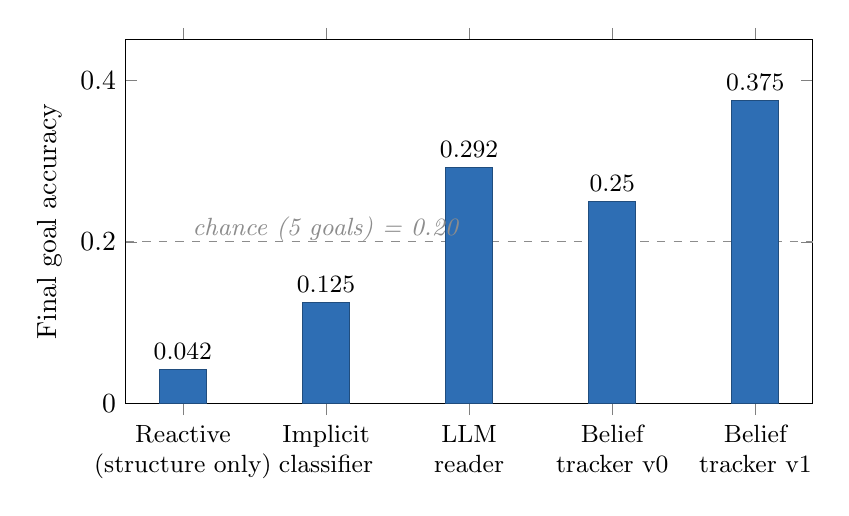
\begin{tikzpicture}
\begin{axis}[
  width=0.85\textwidth, height=6.2cm,
  ybar, bar width=17pt, ymin=0, ymax=0.45,
  ylabel={Final goal accuracy},
  symbolic x coords={Reactive, Implicit, LLM reader, Belief v0, Belief v1},
  xtick=data,
  xticklabels={Reactive\\(structure only), Implicit\\classifier, LLM\\reader, Belief\\tracker v0, Belief\\tracker v1},
  x tick label style={font=\small, align=center},
  nodes near coords, nodes near coords style={font=\small},
  extra y ticks={0.2}, extra y tick labels={},
  extra tick style={grid=major, grid style={dashed, micagray}},
]
\addplot[fill=micablue, draw=micablue!70!black] coordinates {
  (Reactive, 0.042) (Implicit, 0.125) (LLM reader, 0.292)
  (Belief v0, 0.250) (Belief v1, 0.375) };
\node[anchor=west, font=\small\itshape, color=micagray]
  at (axis cs:Reactive, 0.215) {chance (5 goals) = 0.20};
\end{axis}
\end{tikzpicture}
\caption{Final goal accuracy on 24 never-seen real sessions. The reactive
structure-only baseline collapses to 0.042; the belief tracker (v1) reaches
0.375. (Four-arm comparison, cascade of 2026-07-19.)}
\label{fig:necessity}
\end{figure}

\subsection{Claim 2 --- The agent anticipates next movements with minimal context}
\label{sec:claim2}

\textbf{Data.} On 1{,}158 held-out rows from four real sessions fixed by id
before any run, the action decoder's $\tau$-token accuracy (exact for symbolic
tokens, $\pm2$ for coordinates; chance level 0.012 over the 87-token
vocabulary): \textbf{0.710} one action ahead, 0.621 two ahead, 0.586 four
ahead, \textbf{0.593 eight ahead}. On the scripted holdout, the multi-token
retrofit passed its pre-registered adjudication (stage-B NLL $1.637 < 1.660$
stage-A; four-ahead accuracy 0.743).

\textbf{Reading.} ``Minimal context'' is literal: frozen encoders, no
instruction, no goal specification, no labels at deployment --- the decoder
sees only the evidence stream and proposes how the build continues. Predicting
a free human's actions eight steps out at fifty times chance is the strongest
single number in this thesis, and it is the operational meaning of
``understands what the player is doing.''

\subsection{Claim 3 --- Structural understanding accumulates with observation}
\label{sec:claim3}

\textbf{Data.} As the embodied agent's first-person raycast scan covered a real
build (session \texttt{052914}), the shape embedding computed from \emph{only
the scanned cells} converged monotonically to the full structure's embedding:
cosine 0.12 at 9\% coverage $\to$ \textbf{0.92 at 91\% coverage}
(Fig.~\ref{fig:scan}). Independently, the structure matcher scores 1.0 on the
scripted corpus (labels known by construction --- measured, not assumed), and
its free-build boundary is mapped rather than hidden: of 37 labeled real
sessions, 10 matcher-agreed, 18 contested, 9 discarded.

\textbf{Reading.} This is RQ1's positive half with its limits attached: where
ground truth exists the matcher is exact; where builds go off-template it
fails, honestly and measurably --- and that boundary is precisely where
Claim~1 shows the belief must take over.

\begin{figure}[ht]
\centering
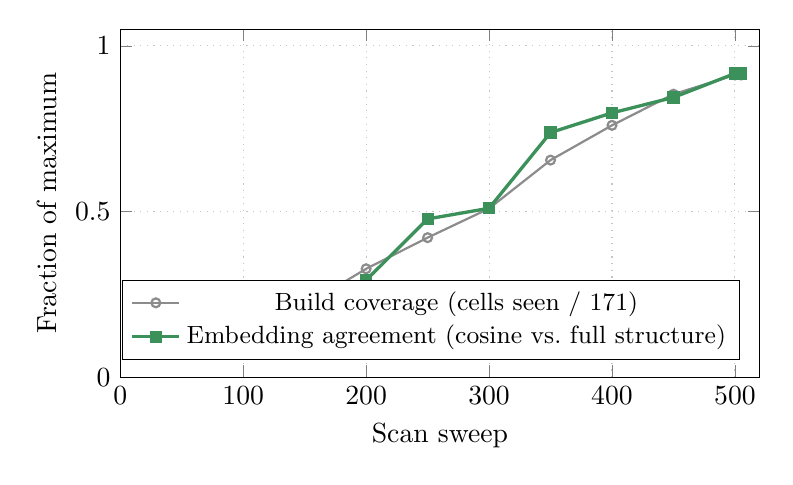
\begin{tikzpicture}
\begin{axis}[
  width=0.8\textwidth, height=6cm,
  xmin=0, xmax=520, ymin=0, ymax=1.05,
  xlabel={Scan sweep}, ylabel={Fraction of maximum},
  legend style={font=\small, at={(0.97,0.05)}, anchor=south east},
  grid=major, grid style={dotted, micagray!50},
]
\addplot[micagray, thick, mark=o, mark size=1.6pt] coordinates {
  (100,0.094) (150,0.216) (200,0.327) (250,0.421) (300,0.509)
  (350,0.655) (400,0.760) (450,0.854) (500,0.912) (505,0.912) };
\addplot[micagreen, very thick, mark=square*, mark size=1.6pt] coordinates {
  (100,0.1165) (150,0.2241) (200,0.2927) (250,0.4775) (300,0.5097)
  (350,0.7382) (400,0.7976) (450,0.8442) (500,0.9164) (505,0.9164) };
\legend{Build coverage (cells seen / 171), Embedding agreement (cosine vs.\ full structure)}
\end{axis}
\end{tikzpicture}
\caption{The agent's partial view carries the full structure's signal: the
embedding of the scanned portion converges to the exact embedding as coverage
grows.}
\label{fig:scan}
\end{figure}

\subsection{Claim 4 --- The system improves lawfully with the right data}
\label{sec:claim4}

Two experiments, both pre-registered with frozen decision rules before any run,
both run inside the same deliberate retrain, both won --- and neither shipped
anything without a separate dated adoption decision.

\textbf{Data (contested labels).} Training the likelihood heads on
matcher-contested sessions with the \emph{builder's} label as truth, against
the agreed-only control, on a shared evaluation set neither arm trained on:
clean accuracy $0.000 \to 0.333$; all-session accuracy $0.182 \to 0.273$;
pooled ECE $0.258 \to 0.232$; sustained-from (build fraction from which the
top goal stays correct; lower = earlier) $0.990 \to 0.897$. All four
pre-registered criteria held. An identical experiment on 2026-07-12 found the
\emph{opposite}; the reversal followed the repair of a feature leak and the
evidence corpus (\S\ref{sec:failed}). Caveat stated with the win: the
evaluation set is 11 sessions.

\textbf{Data (label-free pretraining).} The decoder trained only on scripted
builds was \textbf{1.25 nats worse} on real human action streams than scripted
ones (NLL 3.42 vs.\ 1.77). Because the goal rationale is a separate head
outside the token stream, real sessions --- contested and discarded included
--- can pretrain the next-token stage with zero label-noise risk: real-holdout
NLL fell to \textbf{2.17} ($-37\%$) while the scripted holdout also improved
(1.768 $\to$ 1.725). Real streams were the missing distribution, not noise.

\subsection{A case study, labeled as such}

One live session (the crop farm, Fig.~5 in the figures supplement) shows the
mechanism at work: the belief starts at chance because the live pipeline missed
the first 46 placements, recovers the correct goal from the remaining
evidence, dips honestly when the builder wanders mid-session, and re-locks at
$P=0.84$ as the farm takes shape. Illustrative only; quantitative claims rest
on \S\ref{sec:claim1}.

\section{What failed, and what it taught}
\label{sec:failed}

This section carries the other four claims' credibility.

\textbf{Early recognition is unproven.} The pre-registered criterion ---
sustained correct belief from $\le 40\%$ build progress, significantly above
chance by exact binomial --- fails for \emph{every} arm ($p = 0.058$--$1.0$).
The system recognizes goals mid-build, not early. This is the primary
motivation for more sessions, and goal-recognition-design theory
\cite{grdsurvey} says earliness is partly an environment property --- free
builds may simply not separate goals early.

\textbf{Confidence is not calibrated.} Above 0.4 stated confidence, held-out
reliability \emph{inverts} (the 0.8--0.9 bin hit 6.9\% accuracy) --- Guo et
al.'s overconfidence warning \cite{guo} coming true outside their i.i.d.\
scope. Consequence, taken seriously: the placement threshold sits above the
maximum observed confidence, so confidence-licensed placement is honestly
unreachable until a recalibration stage passes its own pre-registered bar.

\textbf{The belief is not prediction fuel.} A post-hoc probe (labeled as
post-hoc: it was not pre-registered) forced the decoder's intent slot to the
real tracker belief versus an all-zero slot on the real holdout, at horizons
1/2/4/8, on both decoders: \textbf{no gain at any horizon} ($|\Delta| \le
0.001$). The belief is computed from the same evidence the decoder reads, so
for forecasting it is conditionally redundant. Its demonstrated value is
situation classification (Claim~1) and action licensing --- the judgment
layer, not the anticipation layer.

\textbf{A published verdict was reversed --- by finding the bug, not by
re-arguing.} The 2026-07-12 contested-labels experiment concluded the opposite
of \S\ref{sec:claim4}. Between the two runs, an idle-state feature was found
leaking the scoring target into the heads' inputs, and the evidence corpus was
found mis-generated (19 of 25 matcher verdicts changed on regeneration). The
first verdict was honest for its inputs; its inputs were wrong. An interim
results table built on the leaked features was retracted outright.

\textbf{The agent has never assisted.} Across every live session, the agent
placed \emph{zero} blocks (pinned): all authority stayed at suggestion, and
the one acceptance datum collected was \emph{negative} (lift $-0.002$ --- the
unvoiced-proposal control group catching that the builder did the proposed
thing without being told). Assistance in this thesis is designed,
instrumented, and safety-gated --- never evaluated. Given that a confidently
wrong helper is worse than none \cite{wah}, an agent that declines to act
without license is the safety design working, not a shortfall.

\section{Limitations and scope}

Single builder: all real data comes from one person, so there is no
inter-annotator reliability and no cross-player generalization claim. Ground
truth is the builder's own label (defended by design: the matcher's free-build
weakness is documented, and the truth hierarchy --- builder's word outranks
the matcher --- is pinned). No belief-space planning, no environment redesign,
no trained assistance policy: the system only filters, gates, and asks. The
VLM cross-check in the labeling pipeline is diagnostic only; its 94\%
validation number is binary clip agreement with a single annotator and
licenses nothing about five-way judging.

\section{Future work}

(1) \emph{Calibration first}: per-bin recalibration on held-out sessions, with
the pre-registered bar of monotone reliability and pooled ECE $\le 0.15$ ---
the gate to everything else. (2) \emph{Assistance outcomes}: consent-route
sessions with real placements, the acceptance signal at meaningful $n$, and
\textbf{placement survival} (does an agent-placed block remain in the finished
build?) as the outcome measure --- already measurable for free from the
capture's actor-attributed block events. (3) \emph{Earliness}: more sessions
for statistical power, plus the pre-registered hotbar/selection-moment
features (the builder's material choices as pre-placement evidence). (4)
\emph{Transfer}: any domain with discrete observable actions, goals legible
from partial structure, and cheap dense workspace observation.

\section{Conclusion}

An agent can learn to recognize what a person is building and anticipate their
next actions from raw observation alone --- and the intent-inference layer is
what keeps that understanding alive when work stops matching templates. The
equal contribution is the apparatus: pre-registration that constrained its
author, falsification criteria that fired, a leak found and a verdict
reversed in public, and every negative banked beside the positives. That is
what it takes for ``the model understands'' to be a measurement rather than a
slogan.

\begin{thebibliography}{99}\small
\bibitem{cirl} D. Hadfield-Menell, A. Dragan, P. Abbeel, S. Russell.
Cooperative Inverse Reinforcement Learning. \emph{NeurIPS}, 2016.
\bibitem{wah} X. Puig et al. Watch-And-Help: A Challenge for Social Perception
and Human-AI Collaboration. \emph{ICLR}, 2021.
\bibitem{nopa} X. Puig et al. NOPA: Neurally-guided Online Probabilistic
Assistance. \emph{ICRA}, 2023.
\bibitem{assistancezero} C. Laidlaw et al. AssistanceZero: Scalably Solving
Assistance Games. 2025.
\bibitem{carroll} M. Carroll et al. On the Utility of Learning about Humans
for Human-AI Coordination. \emph{NeurIPS}, 2019.
\bibitem{bedd} S. Milani et al. BEDD: The MineRL BASALT Evaluation and
Demonstrations Dataset. \emph{NeurIPS D\&B}, 2023.
\bibitem{vpt} B. Baker et al. Video PreTraining (VPT): Learning to Act by
Watching Unlabeled Online Videos. \emph{NeurIPS}, 2022.
\bibitem{minedojo} L. Fan et al. MineDojo: Building Open-Ended Embodied Agents
with Internet-Scale Knowledge. \emph{NeurIPS}, 2022.
\bibitem{steve1} S. Lifshitz et al. STEVE-1: A Generative Model for
Text-to-Behavior in Minecraft. \emph{NeurIPS}, 2023.
\bibitem{clip4mc} Z. Jiang et al. CLIP4MC: An RL-Friendly Vision-Language
Model for Minecraft. arXiv, 2023.
\bibitem{spatiallm} SpatialLM: Large Language Models for Structured Indoor
Scene Understanding. 2025.
\bibitem{syn2real} X. Peng et al. Syn2Real: A New Benchmark for
Synthetic-to-Real Visual Domain Adaptation. 2018.
\bibitem{apomdp} C.-P. Lam, S. Sastry. A POMDP Framework for Human-in-the-Loop
Systems. \emph{CDC}, 2014.
\bibitem{jainargall} S. Jain, B. Argall. Probabilistic Human Intent
Recognition for Shared Autonomy. \emph{THRI}, 2019.
\bibitem{sips} T. Zhi-Xuan, J. Mann, T. Silver, J. Tenenbaum, V. Mansinghka.
Online Bayesian Goal Inference for Boundedly Rational Planning Agents.
\emph{NeurIPS}, 2020.
\bibitem{clips} T. Zhi-Xuan, L. Ying, V. Mansinghka, J. B. Tenenbaum.
Pragmatic Instruction Following and Goal Assistance via Cooperative
Language-Guided Inverse Planning. \emph{AAMAS}, 2024.
\bibitem{grail} GRAIL: Goal Recognition with Approximated Inference and
Learning. (See vault note for full citation.)
\bibitem{grdsurvey} Goal Recognition Design: A Survey. (See vault note.)
\bibitem{guo} C. Guo, G. Pleiss, Y. Sun, K. Weinberger. On Calibration of
Modern Neural Networks. \emph{ICML}, 2017.
\bibitem{mtp} F. Gloeckle et al. Better \& Faster Large Language Models via
Multi-token Prediction. \emph{ICML}, 2024.
\bibitem{fastscenescript} Yin et al. Fast SceneScript. arXiv:2512.05597.
\end{thebibliography}

\end{document}
